\documentclass{report}

\usepackage[nopdftrailerid=true]{pdfprivacy}
\usepackage{pdfpages}
\usepackage[colorlinks=true,linkcolor=blue,citecolor=blue,urlcolor=blue]{hyperref}
\usepackage[margin=3cm]{geometry}
\usepackage{hyperref}
\usepackage{url}
\usepackage{bytefield}

\usepackage{listings}
\lstset{basicstyle=\ttfamily\small,
    showstringspaces=false,
    commentstyle=\color{blue},
    stringstyle=\color{brown},
    frame=single,
}

\usepackage{mdframed}
\newenvironment{note}[0]    { \begin{mdframed}[backgroundcolor=blue!25]  \textbf{Note:}    \begin{itemize} \itemsep0em } { \end{itemize} \end{mdframed} }
\newenvironment{warning}[0] { \begin{mdframed}[backgroundcolor=red!25]   \textbf{Warning:} \begin{itemize} \itemsep0em } { \end{itemize} \end{mdframed} }
\newenvironment{tip}[0]     { \begin{mdframed}[backgroundcolor=green!25] \textbf{Tip:}     \begin{itemize} \itemsep0em } { \end{itemize} \end{mdframed} }
\newenvironment{exercise}[0]{ \begin{mdframed}[backgroundcolor=yellow!25]\textbf{Exercise:}\begin{itemize} \itemsep0em } { \end{itemize} \end{mdframed} }

\usepackage{tikz}
\usetikzlibrary{arrows,shapes}
\usetikzlibrary{positioning}
\usetikzlibrary{automata}
\usetikzlibrary{petri}
\usetikzlibrary{calc}


\begin{document}

\begin{titlepage}
    \vspace*{5cm}
    \begin{center}
        
\includegraphics[width=0.5\textwidth]{assets/logo-no-background.png}
    \end{center}

    \vspace{1cm}

    \begin{center}
        \textbf{\huge The MOS Project}\\
        \vspace{0.5cm}
        \textbf{\large Lab Tutorial}

        \vspace{5cm}
        Moody Liu\\
        November 2022
    \end{center}
\end{titlepage}

\tableofcontents

\chapter*{Introduction to the MOS Lab}
\addcontentsline{toc}{chapter}{Introduction to the MOS Lab}

\textbf{Welcome to the MOS Lab!}

MOS is a microkernel operating system, it's designed to be simple and easy to understand.
During the lab, you will be working with the MOS kernel and exploring corresponding concepts of
operating systems.

Throughout the labs, you will explore the following topics, in the order listed. Items in
\textbf{bold} are the main topics of the lab, which you may be asked to implement something for.

\begin{itemize}
    \item \textbf{Lab 1}: Development Environment Setup
          \subitem Cross-Compiler Usage
          \subitem Starting the \textbf{QEMU} emulator and attach to it with \textbf{GDB}
    \item \textbf{Lab 2}: Process and Threads
          \subitem \textbf{PCB} \textbf{TCB}, process tables and thread tables
          \subitem \textbf{Creating} a new process
          \subitem \textbf{The famous \texttt{fork()} syscall}
    \item \textbf{Lab 3}: Synchronization
          \subitem \textbf{Synchronization Primitives} such as \textbf{mutex}
          \subitem \textbf{Futex} - Fast User-space Mutex
    \item \textbf{Lab 4}: Memory Management
          \subitem \textbf{Paging}, \textbf{Virtual Memory} and \textbf{Address Spaces}
          \subitem \textbf{Copy-on-Write} and \textbf{Page Fault}
\end{itemize}

\chapter{Lab 1 - Setting Up the Development Environment}

In this lab, we'll set up the basic development environment for the rest of our labs. Firstly
I'll introduce you to the tools and we'll install them, then we'll compile MOS, run it in QEMU
for the first time, and then attach GDB to it.

Finally, and hopefully, you can get your favorite IDE set up to work with MOS.

\section{Introduction to the Tools}

MOS is an operating system, thus, preparing for a development environment is already not
an easy task (bruh). Several efforts have been made to make the process easier.

We are currently targeting the 32-bit \texttt{x86} architecture, the tools in table \ref{tab:tools}
are the ones we'll be using.

\begin{table}[h!]
    \centering
    \begin{tabular}{|l|c|c|}
        \hline \textbf{Tool}               & \textbf{Description}     & \textbf{Installation}            \\
        \hline \texttt{CMake}              & \ref{sec:cmake}          & \ref{sec:cmake-install}          \\
        \hline \texttt{i686-elf} toolchain & \ref{sec:cross-compiler} & \ref{sec:cross-compiler-install} \\
        \hline \texttt{NASM}               & \ref{sec:nasm}           & \ref{sec:nasm-install}           \\
        \hline \texttt{cpio}               & \ref{sec:cpio}           & \ref{sec:cpio-install}           \\
        \hline \texttt{qemu-system-i386}   & \ref{sec:qemu}           & \ref{sec:qemu-install}           \\
        \hline
    \end{tabular}
    \caption{Tools used in this lab}
    \label{tab:tools}
\end{table}

\subsection{CMake} \label{sec:cmake}

\begin{quote}
    CMake is an open-source, cross-platform family of tools designed to build, test and package
    software\footnote{https://cmake.org/}
\end{quote}

MOS uses CMake as the build system generator, it supports many build systems like `Make', `Ninja',
`Visual Studio' and `Xcode'.

\begin{note}
    \item It's the actual build system (e.g. `Make') that starts the compiler, linker, etc.,
    CMake is only to \textbf{generate} the configuration files for such build system.
\end{note}

We'll use `Make' as the build system for MOS in this tutorial, but
\textbf{you can use `Ninja' if you want}.

\subsection{NASM} \label{sec:nasm}

NASM is an assembler for x86 architecture. There are several files under `arch/x86`
that are written in NASM. It has a cleaner syntax than the GNU assembler (i.e. \texttt{as}).

\subsection{cpio} \label{sec:cpio}

Cpio is the format of an archive, and also the tool to create such archives. MOS uses cpio as
the initial root filesystem.

\subsection{qemu-system-i386} \label{sec:qemu}

QEMU is an open-source emulator, it also provides a gdb stub for debugging. It can be
installed via your Linux's package manager.

(e.g. \texttt{apt install qemu-system-i386} or \texttt{pacman -S qemu-system-x86}, \dots).

See its \href{https://www.qemu.org/download}{download page} for more details.

\subsection{i686-elf Toolchain} \label{sec:cross-compiler}

As its name suggests, this is a cross toolchain for `i686-elf' target. `i686' means the 32-bit
x86 architecture, and `elf' is the executable format. They together form the `target-triple' of
the toolchain.

\begin{tip}
    \item Most 64-bit Linux OSes have `target triple' of \texttt{x86\_64-pc-linux-gnu}, or
    \texttt{x86\_64-linux-gnu}.
    \item Read more about `target triple' at \url{https://wiki.osdev.org/Target_Triplet}.
\end{tip}

Unlike other applications (e.g. \texttt{bash} or \texttt{vim}) that they run on an existing
operating system and a standard C library (say, \texttt{glibc} or \texttt{musl}). MOS itself is
the operating system, thus there's not an existing OS for it to run on, neither a standard libc
(i.e. no \texttt{printf}, no \texttt{malloc} etc.) for it to use, considering you're directly
interacting with the CPU and the hardware.

This is called `bare-metal' environment, or `freestanding' environment, a `bare-metal' compiler
toolchain is exactly for this situation.

\begin{warning}
    \item One should never use a hosted compiler (e.g. the \texttt{gcc} installed on the lab machine)
    to cross-compile for a bare-metal environment when they are targeting a different architecture,
    (\texttt{x86} and \texttt{x86\_64} are different), it \textit{\textbf{may sometimes}} work, but
    you'll have to add a lot of unnecessary flags.

    \item See \url{https://wiki.osdev.org/Why_do_I_need_a_Cross_Compiler%3F} for more information.
\end{warning}

\section{Installating the Tools}

\subsection{CMake} \label{sec:cmake-install}

CMake should come with your Linux distribution's package manager, MOS requires at least version
3.20, but any newer version is recommended.

\subsection{NASM} \label{sec:nasm-install}

NASM can be installed via your Linux's package manager, the minimum version of NASM tested is
\texttt{2.15.03}. A pre-built binary from \href{https://www.nasm.us}{NASM's website} is also
available.

\subsection{cpio} \label{sec:cpio-install}

cpio can also be installed via your Linux's package manager, the minimum version of cpio
tested is \texttt{2.12}.

\subsection{qemu-system-i386} \label{sec:qemu-install}

Major Linux distributions provides a package for QEMU, thus it's recommended to install it via
your Linux's package manager.

\subsection{i686-elf Toolchain} \label{sec:cross-compiler-install}

Installing the cross-compiler toolchain is probably the most difficult part of this lab,
but it's once and for all, you don't have to do it again (unless you want to upgrade the
toolchain).

There are majorly two ways to get this toolchain, either by building it from source or by
downloading a pre-built binary.

\subsubsection{Downloading a pre-built binary}

If you don't want to build the toolchain from source, you can download a pre-built
binary from
\href{https://github.com/moodyhunter/i686-elf-prebuilt/releases}{moodyhunter/i686-elf-prebuilt}
(choose the i686 one).

\begin{warning}
    \item Using pre-built binary saves time, but please consider doing so \textbf{only} if
    you trust the author.
    \item The above pre-built binary is built with GitHub Actions, and is built on Ubuntu 20.04.5
    LTS (Image \texttt{ubuntu-20.04} version \texttt{20221027.1}).
\end{warning}

\subsubsection{Building From Source}

The source code of binutils and gcc can be found at
\href{https://www.gnu.org/software/binutils}{GNU Binutils's Website} and
\href{https://gcc.gnu.org}{GNU GCC's Website} respectively.

\begin{note}
    \item For Arch Linux users, checkout
    \href{https://github.com/moodyhunter/repo/blob/main/moody/i686-elf-binutils/PKGBUILD}{i686-elf-binutils},
    \href{https://github.com/moodyhunter/repo/blob/main/moody/i686-elf-gcc/PKGBUILD}{i686-elf-gcc} and
    \href{https://github.com/moodyhunter/repo/blob/main/moody/i686-elf-gdb/PKGBUILD}{i686-elf-gdb}.
\end{note}

The script located at \texttt{docs/assets/i686-elf-toolchain.sh} can download, compile and
install the toolchain into the directory specified by the \texttt{PREFIX} variable.

\section{Building MOS}

\begin{note}
    \item Before you continue reading, make sure \texttt{i686-elf-gcc}, \texttt{i686-elf-ld},
    \texttt{nasm}, \texttt{cpio} are in your \texttt{PATH}.
\end{note}

\subsection{Cloning the Repository}

The recommended way to get MOS is to clone the repository from GitHub:

\begin{verbatim}
    git clone https://github.com/moodyhunter/MOS
    cd MOS
\end{verbatim}

\subsection{Configuring MOS}

If you have a correct setup, then configuring step should be as simple as:

\begin{verbatim}
    $ mkdir build && cd build
    $ cmake ..
\end{verbatim}

The first line creates a build directory, we are not going to build MOS in the source directory
directly, because there will be many generated files, and it's not a good idea to pollute the
source directory.

The second line runs CMake to configure MOS, after running this command, you should see a
bunch of output, similar to \ref{fig:cmake-output}.

\begin{figure}[ht]
    \centering
    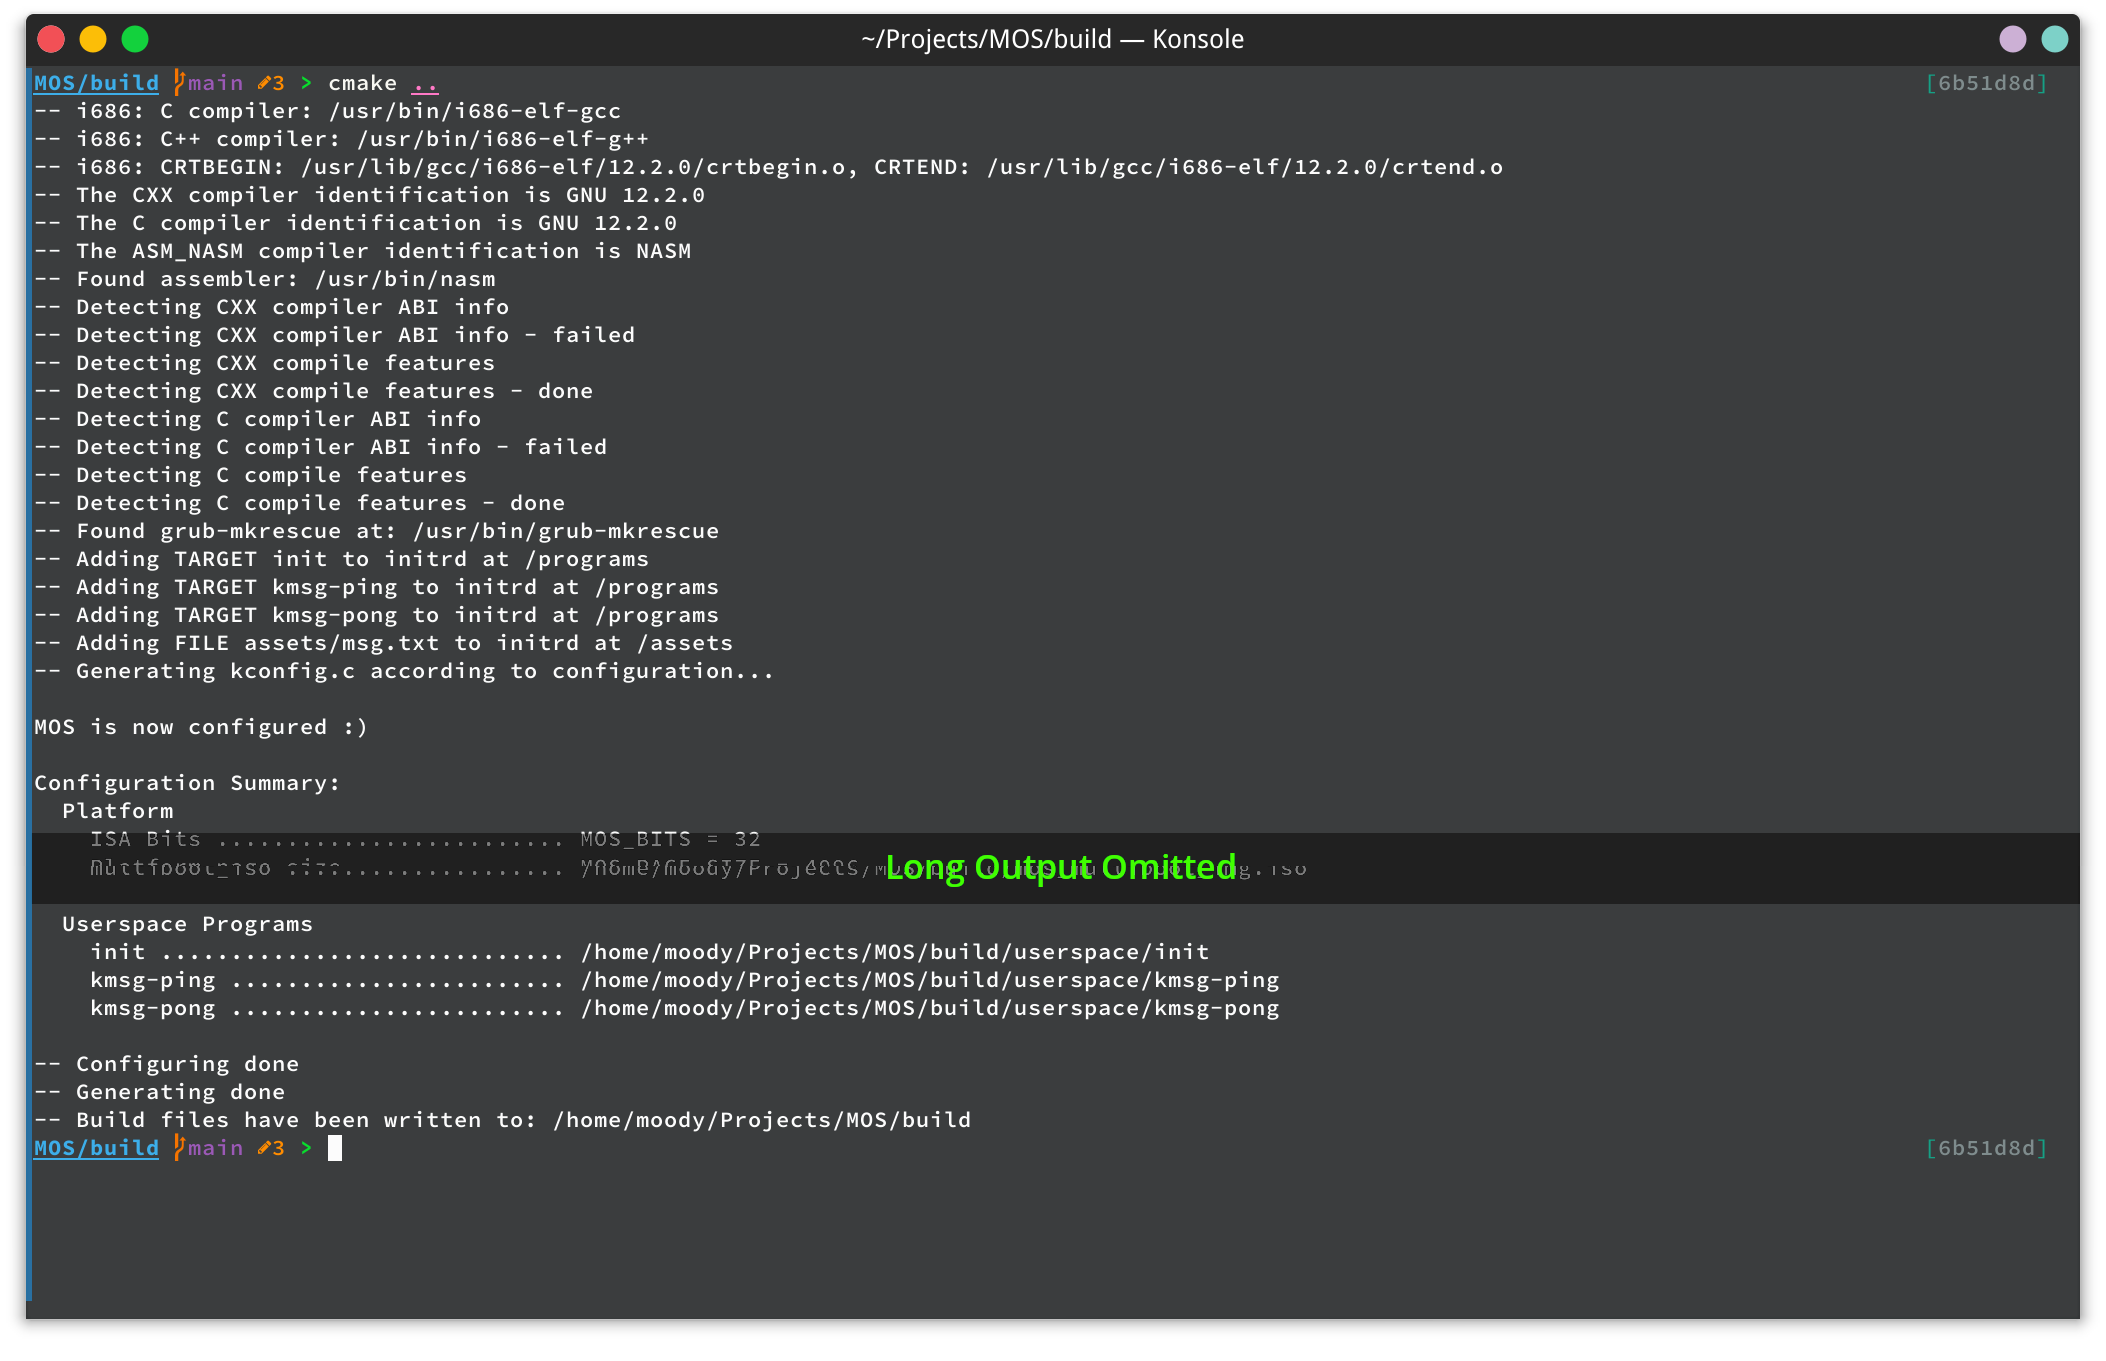
\includegraphics[width=\textwidth]{assets/c1.mos-cmake-configure.png}
    \caption{CMake Output}
    \label{fig:cmake-output}
\end{figure}

Don't worry if you see \texttt{C compiler ABI info} and \texttt{CXX compiler ABI info}
fails, it's because CMake doesn't know what to do with a cross compiler, this check is meaningless.

You may also see \texttt{grum-mkrescue} is not found, don't worry as well :), we are not going to use it.

If you don't see the \texttt{-- Configuring done} or \texttt{-- Generating done} line, then
something has been wrong, and you should scroll up and see what's wrong.

The \texttt{build} directory is where all the generated files are located, you can safely
delete it and re-run CMake to re-generate the files, in case you messed up something.

\subsection{Building MOS}

After configuring MOS, you can build MOS by running \texttt{make}.

This command will only build the core part of MOS, which is the kernel and the userspace library.
See the table below for an example list of targets.

\begin{tip}
    \item Think of a ``target'' as a deliverable, for example, building the \texttt{mos\_kernel} target
    will produce a kernel binary, building the \texttt{mos\_userspace\_programs} will ensure
    all the userspace programs are built.
\end{tip}

\begin{table}[ht]
    \centering
    \small
    \begin{tabular}{|l|l|l|}
        \hline
        \textbf{Target}                   & \textbf{Description}                & \textbf{Depends on}                           \\ \hline
        \texttt{mos\_kernel}              & kernel without boot support         & \textit{None}                                 \\ \hline
        \texttt{mos\_initrd}              & The Initial RAMDisk Image           & \texttt{mos\_userspace\_programs}             \\ \hline
        \texttt{mos\_userspace\_programs} & Userspace programs                  & \texttt{init}, other userspace programs \dots \\ \hline
        \texttt{init}                     & The init program                    & \dots                                         \\ \hline
        \texttt{multiboot}                & \texttt{multiboot} compatible image & \texttt{mos\_kernel}                          \\ \hline
    \end{tabular} \\
    \begin{note}
        \item This is not a complete list.
        \item For a complete list of targets, run \texttt{make mos\_print\_summary} or \texttt{ninja mos\_print\_summary}
        and observe the ``\texttt{Userspace Targets}'', ``\texttt{Utility Targets}'' and ``\texttt{Bootable Targets}'' sections.
    \end{note}
    \caption{Targets}
    \label{tab:targets}
\end{table}

We are going to build the \texttt{multiboot} and \texttt{mos\_initrd} targets, these are the two
`utility' targets that 1) produce a bootable kernel and 2) create an initrd image.

An `initrd' is a compressed archive that contains our userspace programs, it literally means ``initial ramdisk'',
that is, the disk image that is loaded into the RAM when the kernel boots.

So the command will be \texttt{make multiboot mos\_initrd} (replace \texttt{make} with \texttt{ninja} if you are using Ninja).

You'll then see two files being generated in the \texttt{build} directory:

\begin{itemize}
    \item \texttt{mos\_multiboot.bin} is the kernel image, which is a multiboot-compliant kernel.
    \item \texttt{initrd.cpio} is the initrd image, which contains the userspace programs.
\end{itemize}

Several other files are also generated, for more information, read the MOS documentation, section \texttt{CMake Targets}.

\begin{exercise}
    \item Use the utility target \texttt{mos\_print\_summary} to print a summary of all the targets.
    \item Navigate to \texttt{initrd} under the build directory, and use \texttt{find .} to list all the files.
\end{exercise}

\section{Running MOS}

Once we have compiled MOS, we can run it in QEMU.

The command passed to QEMU will be flexible based on your needs, but the most basic command is:

\begin{verbatim}
    qemu-system-i386 -m 4G -kernel mos_multiboot.bin -initrd initrd.cpio -serial stdio
\end{verbatim}

You can pass more arguments to QEMU:

\begin{itemize}
    \item \texttt{-s} to enable the QEMU GDB stub, which allows you to debug MOS using GDB.
    \item \texttt{-S} to pause the CPU before starting up, which allows GDB to take control of
          the booting process.
    \item \texttt{-m} to specify the amount of RAM to be allocated to the VM (say \texttt{-m 512M}).
          the preferred amount of RAM is 4GB, less RAM may cause the kernel to fail.
    \item \texttt{-append} to pass arguments to the kernel, several arguments are:
          \begin{itemize}
              \item \texttt{quiet}: suppress (most-of) all non-warning kernel messages.
              \item \texttt{init=}: path to the init program, e.g. \texttt{init=/initrd/programs/mossh}.
          \end{itemize}
          For a complete list of supported arguments, see the MOS documentation section.
    \item \dots For more possible arguments, you may want to read QEMU's documentation.
\end{itemize}

\begin{tip}
    \item If you accidentally specified \texttt{-nographic} to QEMU and find that you can't terminate
    the QEMU process by pressing \texttt{Ctrl+C}. You can press \texttt{Ctrl+A} and then \texttt{x}
    instead to achieve the same effect. (Press \texttt{Ctrl+A} and then \texttt{h} to see a list of these
    shortcuts.)
\end{tip}

\begin{exercise}
    \item Run MOS with the command above.
    \item Run MOS with \texttt{-m 3G} and \texttt{-m 512M}, what's the difference?
\end{exercise}

\section{Debugging MOS}

After successfully building and running MOS, you may want to debug it (just in case your code crashes
the kernel).

\subsection{Required QEMU Arguments} \label{sec:qemu-args}

As mentioned above, we need to pass 2 more arguments \texttt{-s} and \texttt{-S} to QEMU so that it
1) enables the GDB stub, and 2) pauses the CPU before starting up (so that we have time to attach and
place breakpoints).

After adding these two arguments, when starting up QEMU, you will see a message like Figure \ref{fig:qemu-gdb-paused}.

\begin{figure}[h]
    \centering
    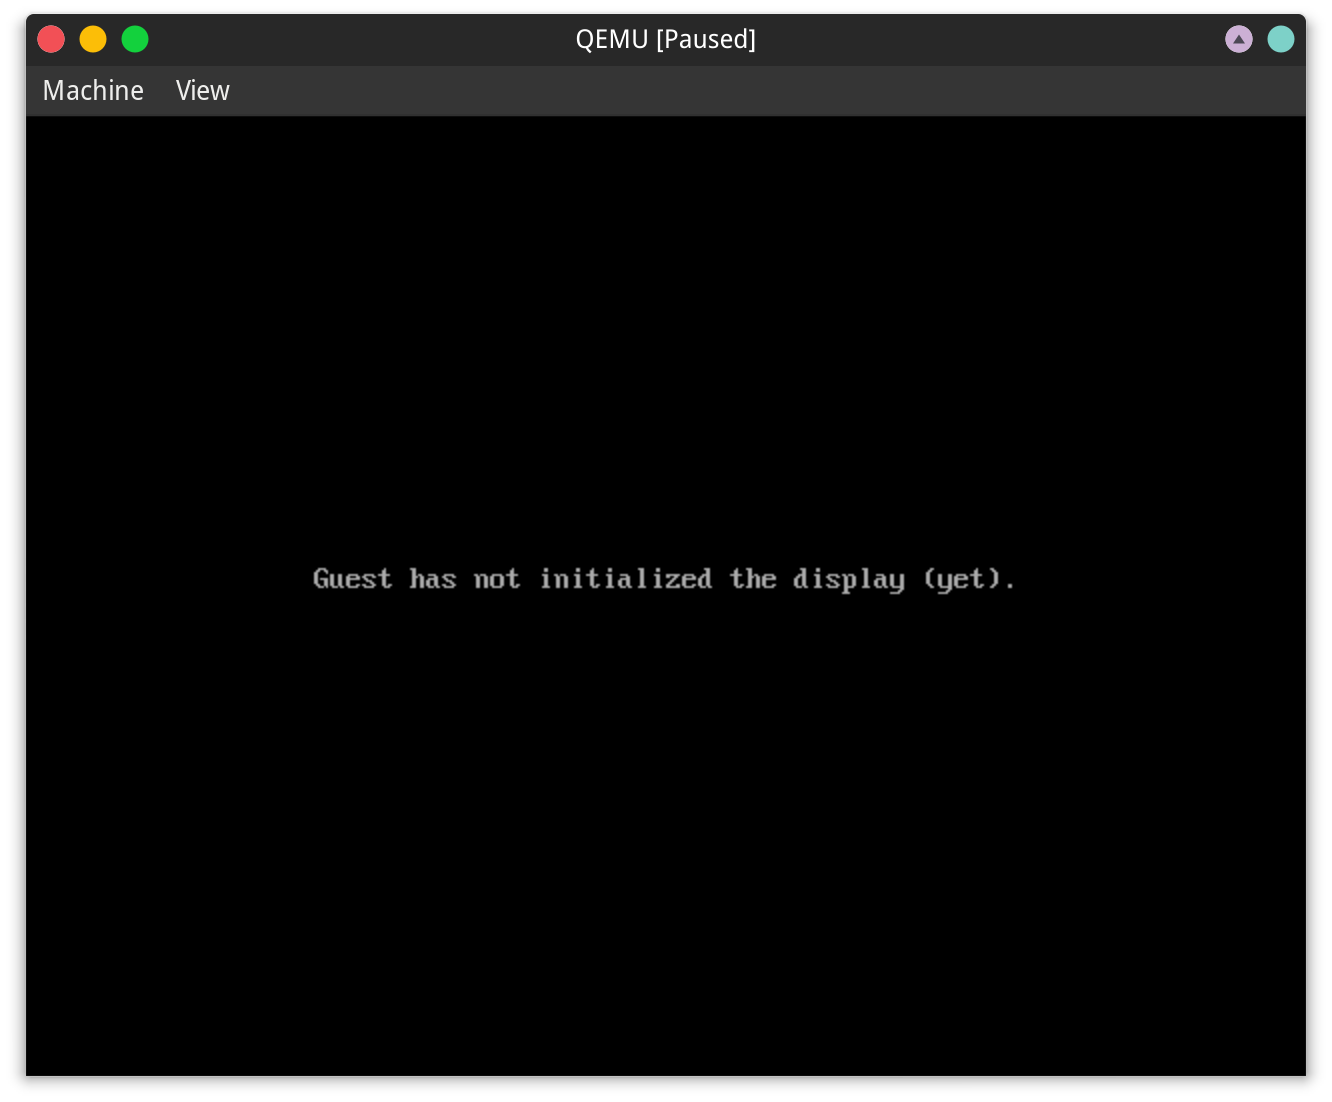
\includegraphics[width=\textwidth]{assets/c1.mos-qemu-gdb-paused.png}
    \caption{QEMU GDB in Paused State}
    \label{fig:qemu-gdb-paused}
\end{figure}

This means that QEMU is waiting for a GDB connection, and we can now continue to the next step.

\subsection{Configuring GDB} \label{sec:gdb-config}

Note that we are targeting the \texttt{i686-elf} architecture, so you should use \texttt{i686-elf-gdb}
instead of \texttt{gdb}.

To begin with, we need to tell GDB where the kernel file is, so that GDB can load debug information
from it.

You've probably already seen a \texttt{gdbinit} file in the \texttt{build} directory. This file
contains commands for GDB to recognize our userspace programs, we'll pass this file to GDB using
the \texttt{-x} argument.

So the overall command will be:

\begin{verbatim}
    i686-elf-gdb ./mos_multiboot.bin -x ./gdbinit
\end{verbatim}

\subsection{Attaching to QEMU} \label{sec:gdb-attach}

After GDB starts, you'll see it's `adding symbol table from file' thanks to our \texttt{gdbinit} file.
Now we need to attach GDB to QEMU, so that we can place breakpoints and debug the kernel.

QEMU (by default) listens on port 1234 for GDB connections, so we need to tell GDB to connect to it:

\begin{verbatim}
    (gdb) target remote localhost:1234
\end{verbatim}

GDB will then connect to QEMU, and you'll see a message like Figure \ref{fig:gdb-attached}.

\begin{figure}[ht]
    \centering
    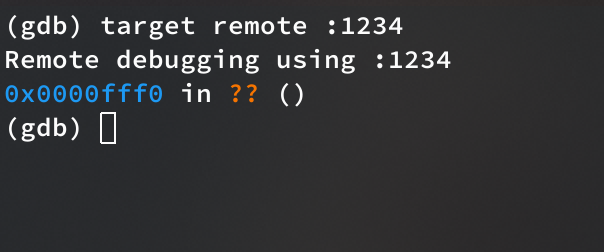
\includegraphics[width=\textwidth]{assets/c1.gdb-attached.png}
    \caption{GDB Attached to QEMU}
    \label{fig:gdb-attached}
\end{figure}

Try typing \texttt{break main} and then \texttt{continue} to see if it pauses at the \texttt{main}
function, you should see a message like Figure \ref{fig:gdb-paused}.

\begin{figure}[ht]
    \centering
    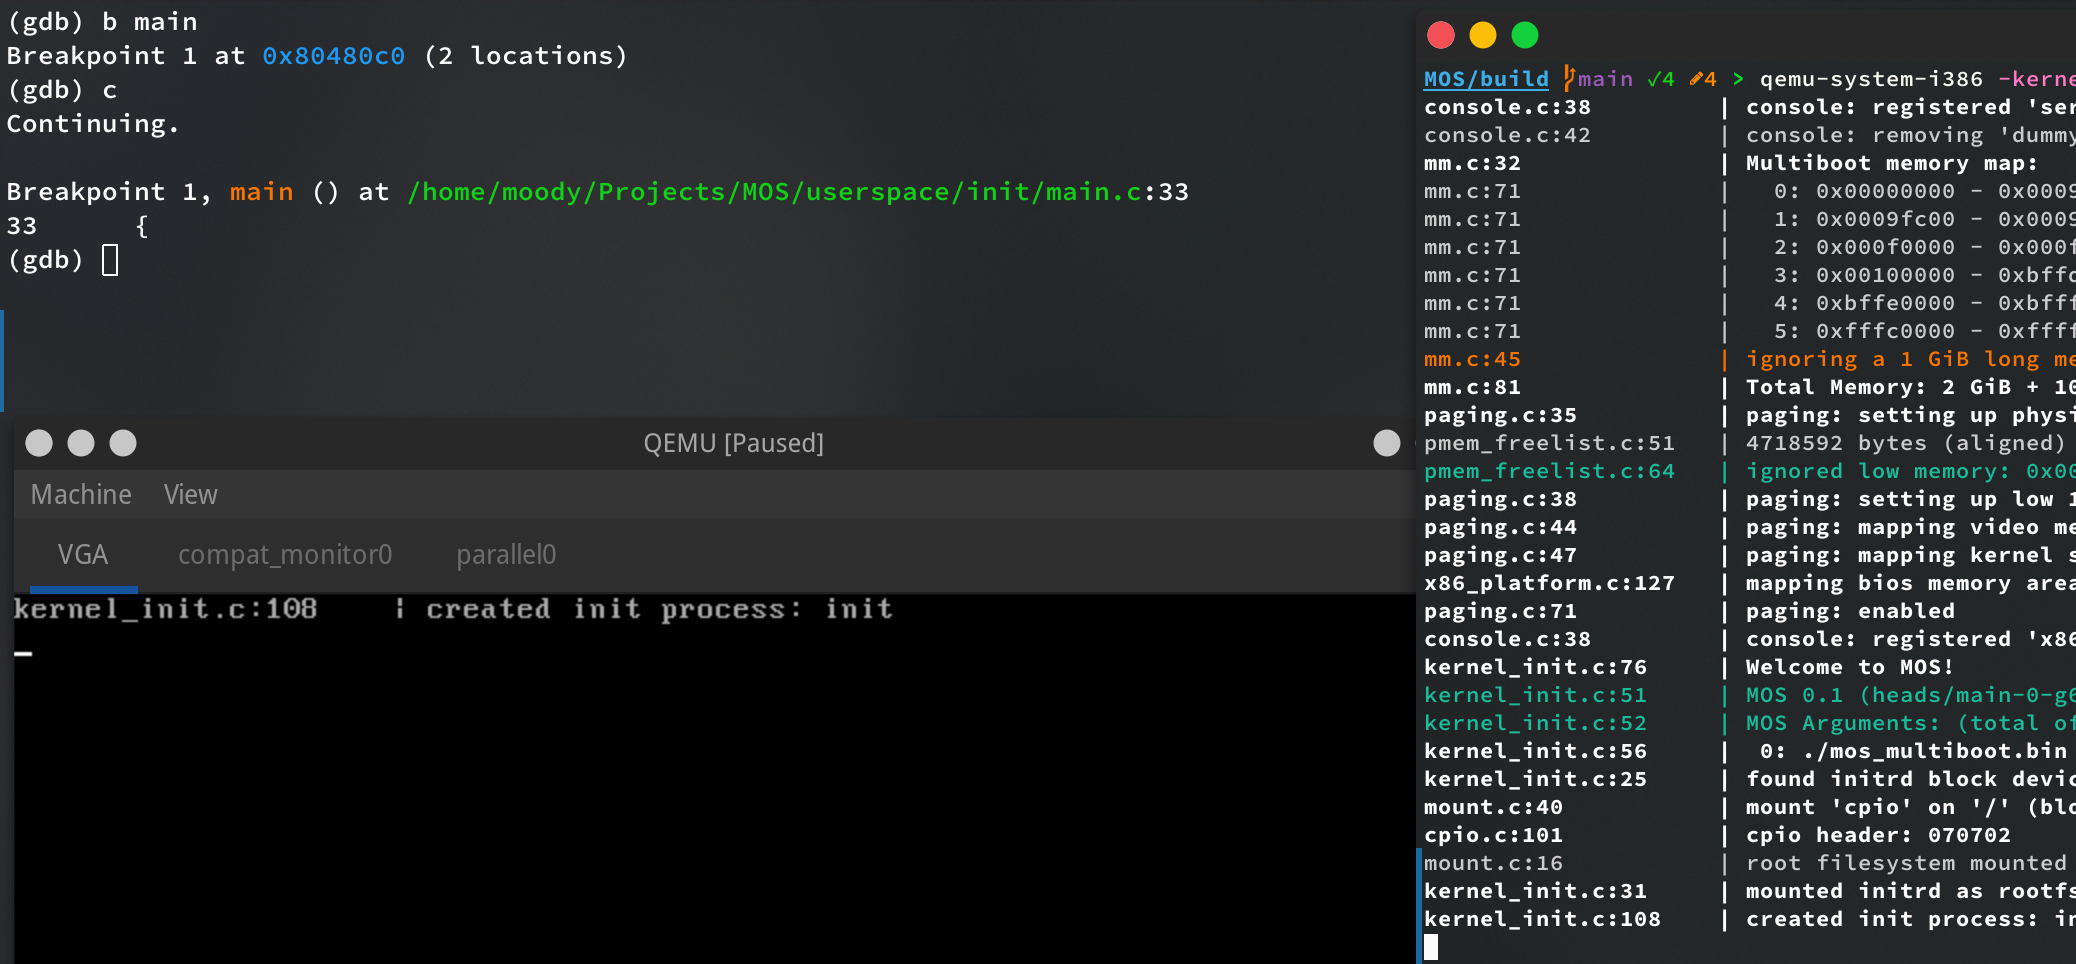
\includegraphics[width=\textwidth]{assets/c1.gdb-paused.png}
    \caption{GDB Paused at \texttt{main}}
    \label{fig:gdb-paused}
\end{figure}

\subsection{(Optional) Configure your IDE for Future Debugging} \label{sec:ide-config}

\begin{note}
    \item I personally use VSCode, thus only the VSCode part will be covered here. If you are
    using any other IDE (e.g. CLion), things \textbf{may} be different, but the underlying idea
    of remote debugging should be the same.

    \item IDEs are updating very fast, so the screenshots \textbf{may} be outdated. Ask me if you
    have any questions.
\end{note}

As you may (or may not) realize, attaching GDB to QEMU is basically same as remote debugging, so
we can configure our IDE to do this automatically. But notice that:

\begin{itemize}
    \item Use \texttt{i686-elf-gdb} instead of the default \texttt{gdb}
    \item We need to specify the \texttt{gdbinit} file.
\end{itemize}

\subsubsection{Prepared VSCode Setup} \label{sec:vscode-config}

\begin{tip}
    \item There are several suggested VSCode extensions:
    \begin{itemize}
        \item \texttt{C/C++} for C/C++ support
        \item \texttt{clangd} for C/C++ language server
        \item \texttt{CMake} for CMake support
    \end{itemize}
    \item \texttt{tmux} is also required for this setup.
\end{tip}

To use a prepared setup for VSCode, see the \texttt{launch.json} file in the \texttt{.vscode}
directory, which is also my personal configuration for debugging MOS.

Simply press \texttt{F5}, a QEMU window will pop up and you'll see the kernel booting up, with
the breakpoints you set in your IDE as shown in Figure \ref{fig:vscode-debugging}.

In this setup, you can also use \texttt{tmux attach-session -t mos\_kernel\_debug} to attach to the serial
port.

\begin{figure}[ht]
    \centering
    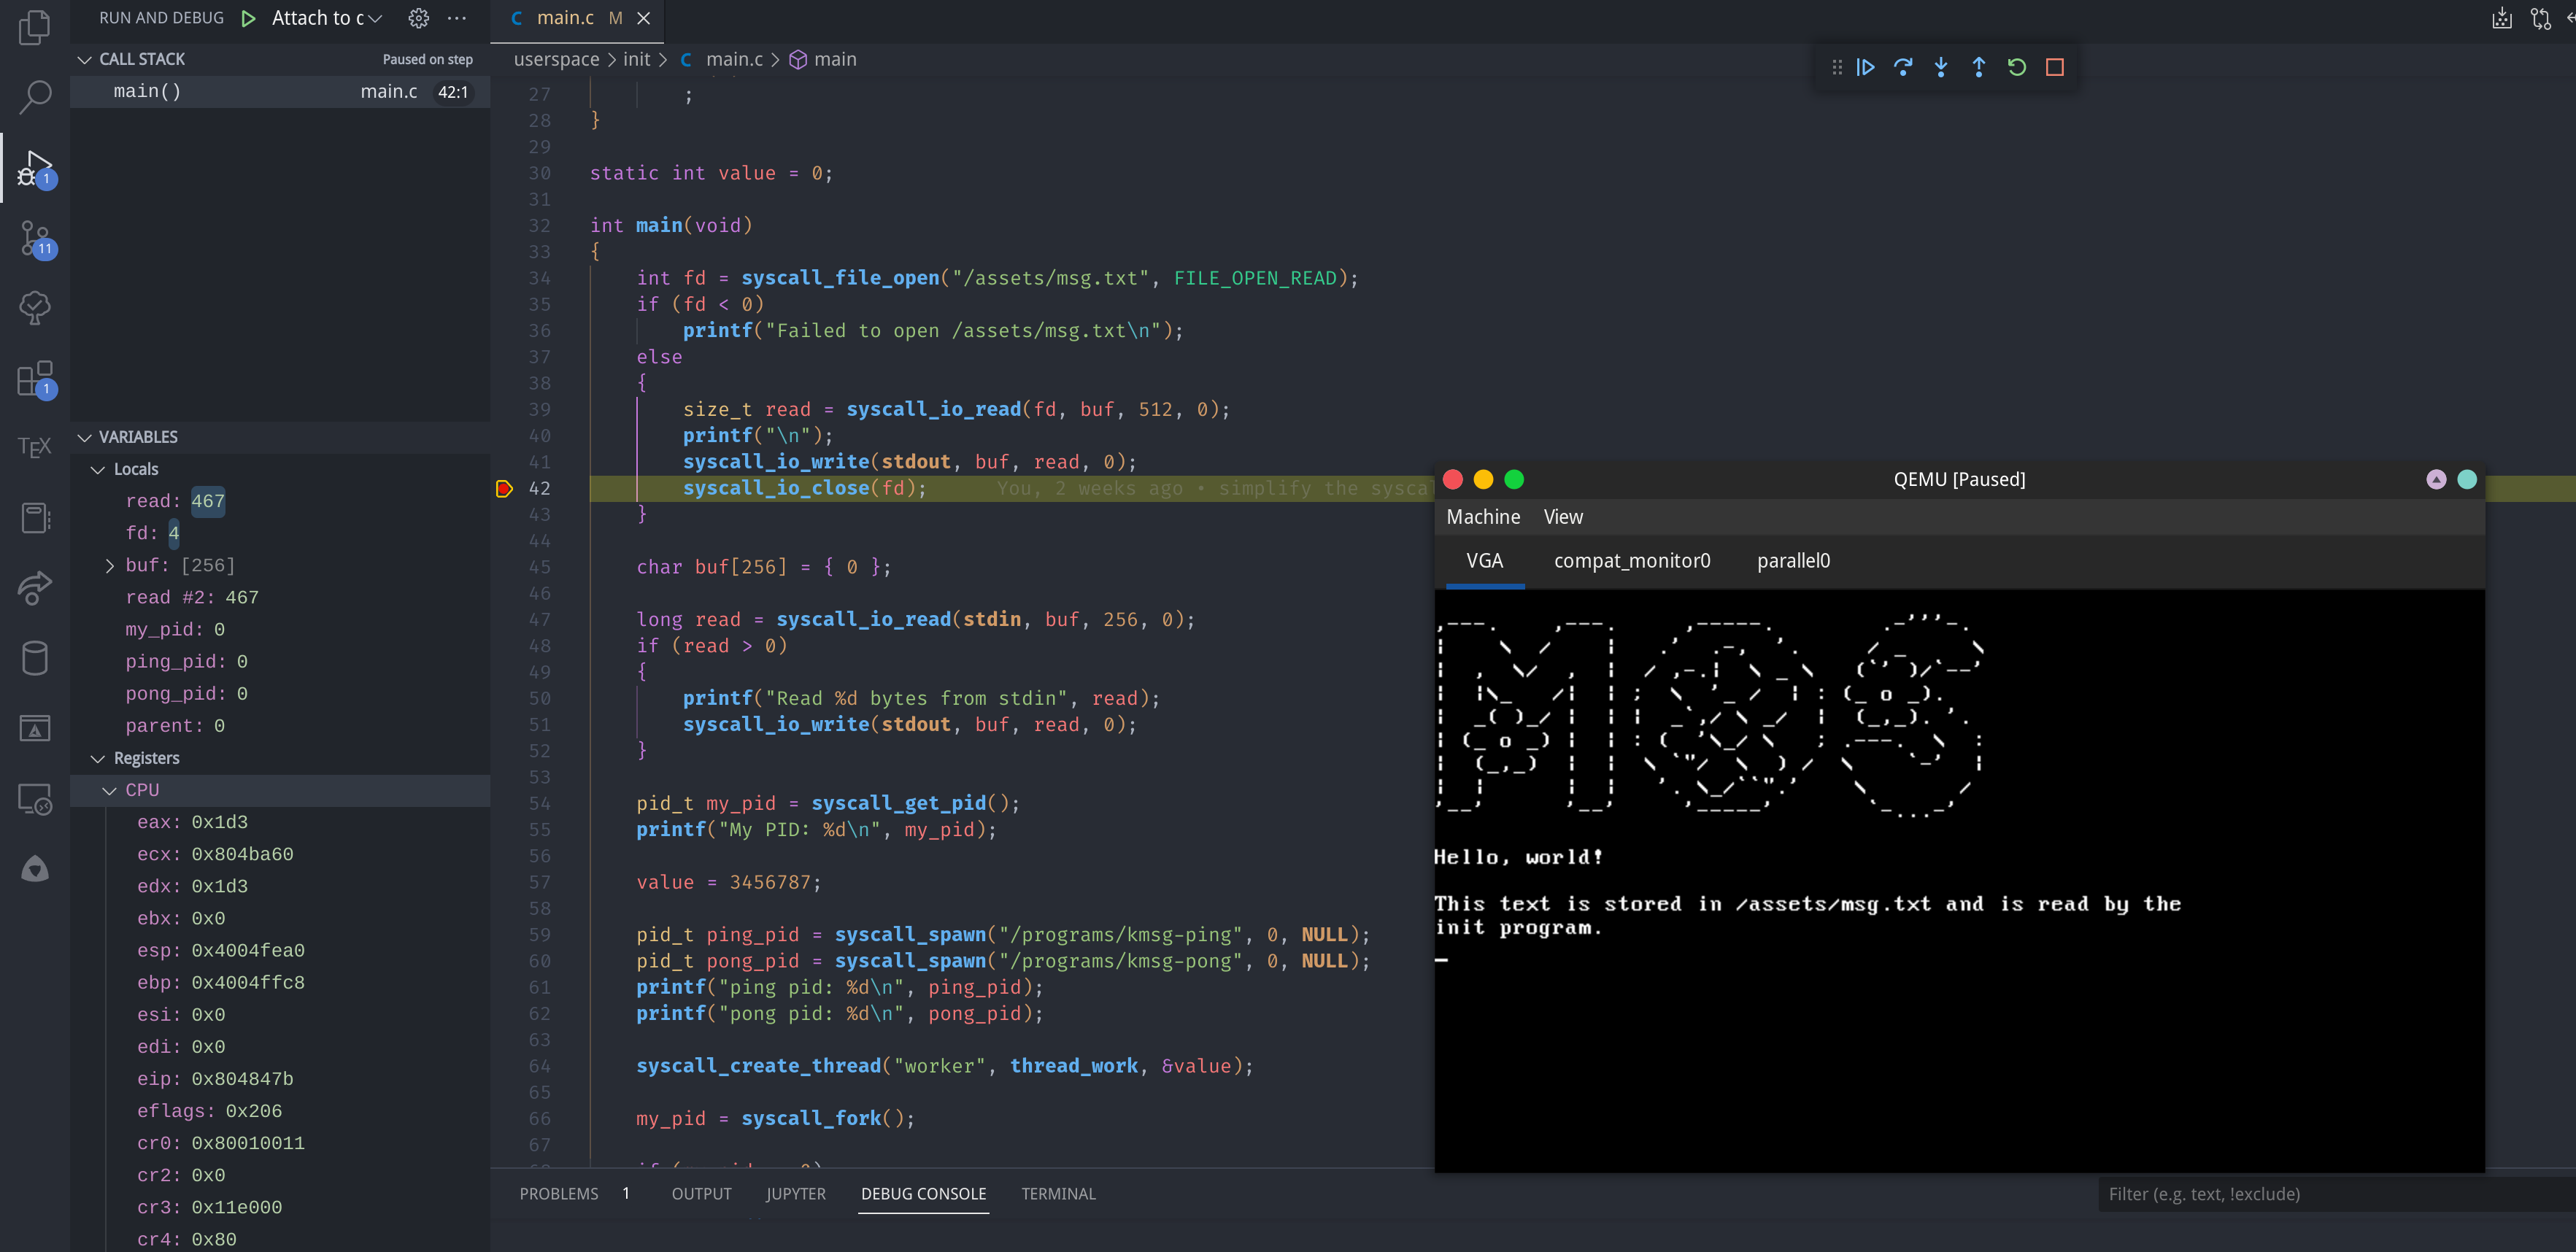
\includegraphics[width=\textwidth]{assets/c1.vscode-debugging.png}
    \caption{VSCode Debugging MOS}
    \label{fig:vscode-debugging}
\end{figure}

\subsection{Summary}

In this section, we've configured the cross-compiler, the build system and (possibly) the IDE for
our future MOS kernel development. We've also learned how to debug MOS kernel using QEMU and GDB.

Below are some exercises for you to practice and test your environment setup.

\begin{exercise}
    \item In the \texttt{mos\_start\_kernel} function (in \texttt{kernel/kernel\_init.c}), you'll find
    texts like `Welcome to MOS!'. Add some code here to print out your name with some other information.
    e.g. `This is [YOUR NAME]'s own version of MOS!'

    Compile and run the kernel, do you see your name printed out?

    \begin{tip}
        \item There are various ways to print out strings in MOS kernel, you can either of:
        \texttt{printk}, \texttt{pr\_info}, \texttt{pr\_info2}, \texttt{pr\_emph}, \texttt{pr\_warn},
        \texttt{pr\_emerg} or \texttt{pr\_fatal}, they have similar usage like \texttt{printf}.
        \item Can you spot the difference between \texttt{pr\_info} and \texttt{pr\_info2}?
    \end{tip}

    \item Try to set a breakpoint somewhere in the \texttt{mos\_start\_kernel} function, start debugging
    the kernel and see if it works.

    \item Optionally, try play with different CMake options, like \texttt{MOS\_DEBUG\_ALL}. See what happens to the
    kernel log.
\end{exercise}

\chapter{Lab 2 - Processes}

Congratulations on completing the first lab! Hopefully, you have had a chance to play
around with the MOS kernel and have a better understanding of its structure.

In this lab, we will be looking at the process management in MOS.

\section{Files in MOS that relate to process management}

\begin{figure}[ht]
    \centering
    \raisebox{-.5\height}{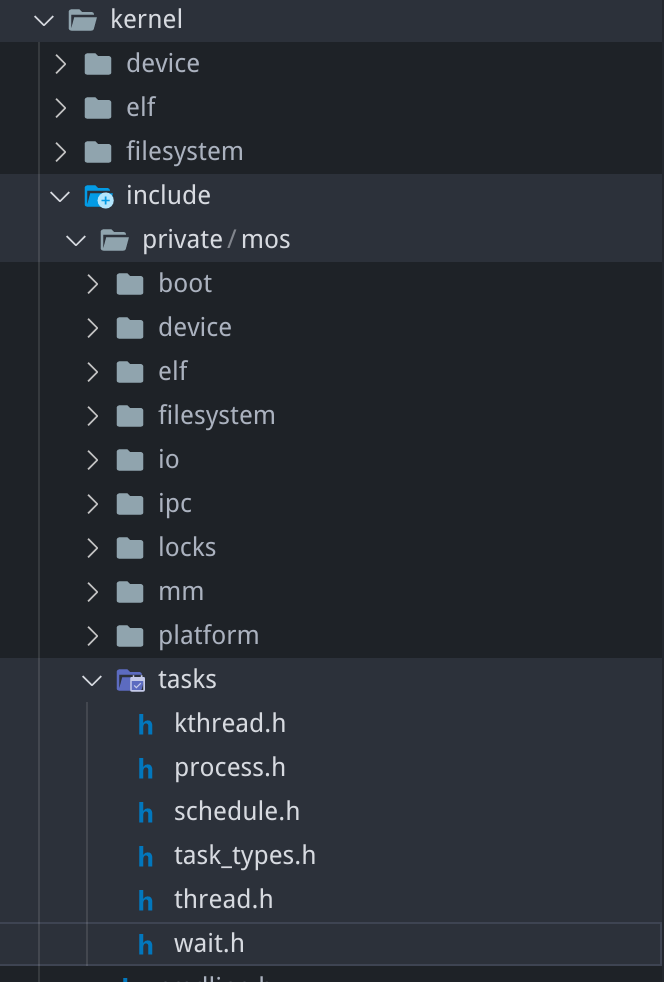
\includegraphics[width=0.4\textwidth]{assets/c2.headers.png}}
    \raisebox{-.5\height}{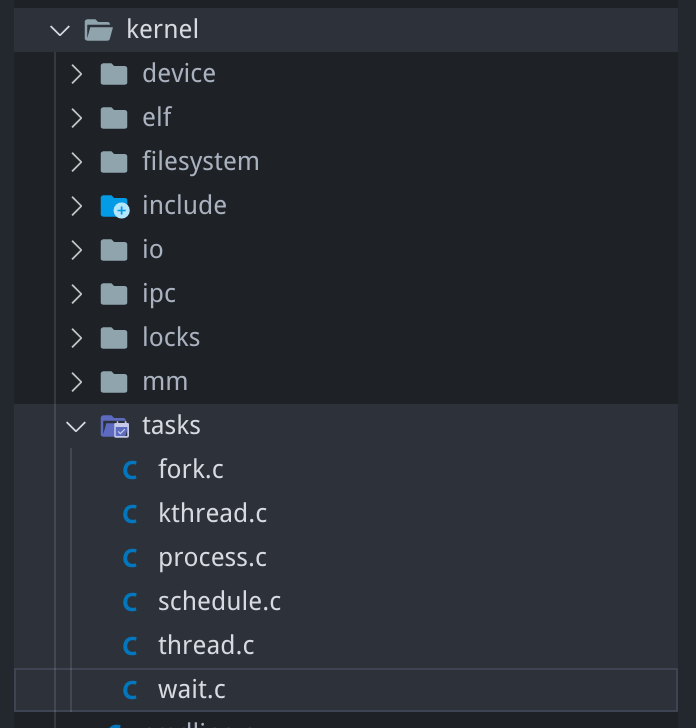
\includegraphics[width=0.4\textwidth]{assets/c2.sources.png}}
    \caption{The header and source files in \texttt{kernel/tasks}}
    \label{fig:mos-process-management-files}
\end{figure}

The process management in MOS is implemented in the \texttt{kernel/tasks} directory and the
corresponding header files are in \texttt{kernel/include/private/mos/tasks} as shown in
Figure \ref{fig:mos-process-management-files}.

\begin{note}
    \item The \texttt{kernel/include/private} directory is a convention used in MOS, which
    contains the header files that are \textbf{not} meant to be used by userspace programs.
\end{note}

\section{Process Control Blocks}

You have learnt about this in the lecture: `a process is a program in execution', and a process
control block (PCB) is a data structure that contains information about a process.

Now, let's look at the PCB structure in MOS. The PCB is defined as a struct named \texttt{process\_t}
in \texttt{task\_types.h}.

Several fields are defined in PCB, but we will only look at the ones that are relevant to
process management, they are:

\begin{itemize}
    \item \texttt{pid}: The process id.

          Each process has a unique id, this is what MOS uses to identify a process.\\
          In MOS, the process id is an unsigned 32-bit integer, and this number always
          increases.

    \item \texttt{name}: The name of the process, nothing interesting here.

    \item \texttt{parent}: The parent of the process, this is a pointer to the PCB of the parent.

          Unlike most animals, a process can only have one parent. The \texttt{init}
          process lives at the root of the process tree, it's fun to think about it being its own
          parent.

    \item \texttt{files}: A list of opened files.

          This is a statically allocated array of size \texttt{MOS\_PROCESS\_MAX\_OPEN\_FILES},
          the value of which is determined by the kernel configuration.

          Each time a file is opened, an \texttt{io\_t} that represents an IO object (file, pipe, etc.)
          is added to this array, and the index of such an object is returned to the user program.

          This index is called a `file descriptor', or `fd' for short. The user program can use
          this number to refer to the file in the future.

          The \texttt{io\_t} structure is defined in \texttt{kernel/include/private/mos/io/io.h},
          details of which are probably beyond the scope of this lab.

    \item \texttt{threads}: A list of threads.

          To be honest, this list is unnecessary, because we already have a thread table elsewhere
          in MOS, the list here is just a convenience for the kernel to iterate over all threads
          of a specific process, (think about it as a cache).

    \item \texttt{pagetable}, \texttt{mmaps}: The page table and a list of mapped memory regions,
          these two will be discussed in later chapters.
\end{itemize}

\section{Thread Control Blocks}

You may have noticed that the PCB above is \textit{a little bit} different from the one in the
lecture: It has neither `process state' nor `stack/heap/text memory regions'.

Because, in MOS, a thread is the basic unit of execution instead of a process. Thus it's the thread that has a
`state' and a `stack', and the process is just a collection of threads.

The thread control block is defined in the same file as the PCB. You can see that it contains
a \texttt{tid} for a thread id, a \texttt{state} field to indicate the state of the thread,
its owner process, and two stacks for the kernel and user mode respectively. There's also a
\texttt{context} pointer, this will be used in context switching, we'll look at that later.

\section{Process Creation}

To create a process, the following steps are taken:

\begin{enumerate}
    \item Load the program into the memory.
    \item Create a PCB and populate the fields.
          \begin{enumerate}
              \item Allocate and initialize the PCB.
              \item Allocate a user-mode page table.
              \item Parse the program and map corresponding memory regions into the page table.
              \item Allocate a heap for the process in the user-mode page table.
                    (part 2 in Figure \ref{fig:mos-process-memory-layout})
              \item Add the PCB to the process table.
          \end{enumerate}
    \item Create a main thread.
          \begin{enumerate}
              \item Allocate and initialize the TCB for the main thread.
              \item Allocate \textbf{both} the user-space and kernel-space stack space for the thread.
                    (part 2 in Figure \ref{fig:mos-process-memory-layout})
              \item Add the thread to the thread table.
              \item Set thread state to \texttt{CREATED}.
          \end{enumerate}
    \item (optionally) schedule to the new thread.
\end{enumerate}

A process has to be created from a `program' (an executable file) in order to be executed.
In MOS, the format called `ELF' is used as the executable format.

Thus, to be honest, the journey of a process should start from the function \texttt{elf\_create\_process}
located in \texttt{kernel/elf/elf.c} (corresponding to the first step above), but the code for
parsing an ELF file is a bit overcomplicated and not very interesting.

Because of that, we'll jump ahead and begin at the \texttt{process\_new} function.

\subsection{\texttt{process\_new}}

This function is defined in file \texttt{kernel/tasks/process.c}. It accepts several arguments,
the important ones among them are:

\begin{itemize}
    \item \texttt{process\_t *parent}: The parent of the process, this is a pointer to the PCB of the parent.
    \item \texttt{const char *name}: The name of the process, this is just a string that is used for debugging.
    \item \texttt{thread\_entry\_t entry}: The entry point of the process, this is the address of the
          \texttt{main} function of the program.
\end{itemize}

The function first allocates a PCB by calling \texttt{process\_allocate}. In that function, a
\texttt{process\_t} structure is allocated and initialized. The PID, magic number, name and
parent are set, and then it calls \texttt{mm\_create\_user\_pgd} to create a user-mode page table,
which will become the `address space' of the process.

Going back to \texttt{process\_new}, several (precisely, 3) calls to \texttt{process\_attach\_ref\_fd}
are made to attach the standard input, output and error streams to the process.

Then the function calls \texttt{thread\_new} to create a main thread for the process. As you can see,
the \texttt{entry} is passed as the argument.

\begin{note}
    \item The function also passes \texttt{NULL} as the \texttt{arg} argument, which is an implementation
    detail that MOS handles arguments for the main thread differently.
\end{note}

After the main thread is created, the function allocates a heap by calling \texttt{mm\_alloc\_pages}
and then completing the initialization of the PCB by adding the PCB to the process table.

We'll now look at the \texttt{thread\_new} function.

\subsection{\texttt{thread\_new}}

This function is defined in file \texttt{kernel/tasks/thread.c}.

Similarly, it first calls \texttt{thread\_allocate} to allocate a TCB for the thread, which
initializes the \texttt{tid}, \texttt{magic}, \texttt{owner}, \texttt{state} and \texttt{mode}
fields.

After a TCB is allocated, the function allocates two types of stacks for the thread:

\begin{itemize}
    \item \textbf{Kernel Mode Stack}

          This is the stack used when the thread is running in kernel mode. A thread is running
          in `kernel mode' when it is executing a system call, or when a hardware interrupt, such as
          a timer interrupt or a keyboard interrupt, occurs.

    \item \textbf{User Mode Stack}

          This is the stack used when the thread is running in user mode, nothing special here.
\end{itemize}

\begin{tip}
    \item Pay attention to the different \texttt{mm\_} functions used to allocate the stacks.
    The kernel stack is allocated by \texttt{mm\_alloc\_pages}, while the user stack is
    allocated by \texttt{mm\_alloc\_zeroed\_pages}.
    \item The reason for this will be explained in the later chapters.
\end{tip}

After stacks are allocated, the function calls \texttt{platform\_context\_setup}, which is
a platform-specific function that sets up the initial context of the thread.

Although we won't go into details about architecture-specific code, it's worth noting it's here
that the \texttt{entry} and \texttt{arg} arguments are used. For example, the entry will be
the initial instruction pointer of the thread and the \texttt{arg} will be pushed onto the stack
or passed in a register (depending on the architecture).

After the context is set up, the function adds the thread to the thread table, completing
the initialization of that thread.

\subsection{Thread States}

In MOS, a thread can be in one of the following states:

\begin{itemize}
    \item \texttt{CREATED}: thread is created or forked, but not ever started
    \item \texttt{READY}: thread can be scheduled
    \item \texttt{RUNNING}: thread is currently running
    \item \texttt{BLOCKED}: thread is blocked by a wait condition
    \item \texttt{DEAD}: thread is dead and will be cleaned up soon by the scheduler
\end{itemize}

The state transition diagram of a thread is shown in Figure \ref{fig:thread-state-transition}
\footnote{Process termination with multiple running threads is not shown in this diagram}.

\begin{figure}
    \centering
    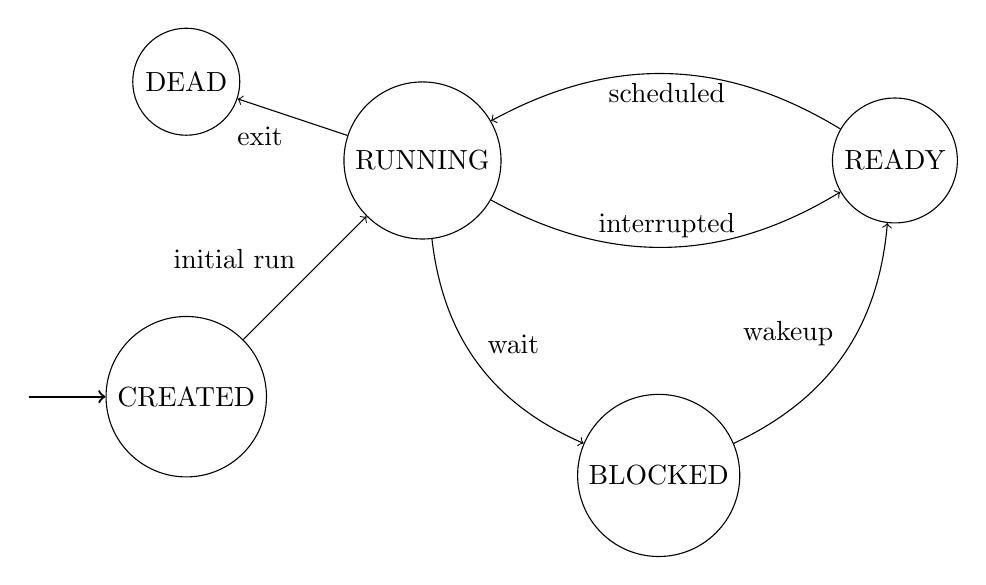
\begin{tikzpicture}[auto]

        \node[state] (C) at (0,-2) {CREATED};
        \node[state] (D) at (0, 2) {DEAD};

        \node[state] (U) at (3, 1) {RUNNING};
        \node[state] (R) at (9, 1) {READY};
        \node[state] (B) at (6,-3) {BLOCKED};

        \draw[->, thick] (-2, -2) -- (C);

        \path[->] (C) edge node {initial run} (U);
        \path[->] (U) edge node {exit} (D);

        \path[->] (U) edge [bend right] node {interrupted} (R);
        \path[->] (R) edge [bend right] node {scheduled} (U);
        \path[->] (U) edge [bend right] node {wait} (B);
        \path[->] (B) edge [bend right] node {wakeup} (R);
    \end{tikzpicture}
    \caption{Thread State Transition Diagram in MOS}
    \label{fig:thread-state-transition}
\end{figure}

\begin{note}
    \item MOS transitions a thread from \texttt{CREATED} \textbf{directly} to
    \texttt{RUNNING} without going through the \texttt{READY} state. This is different
    from what's in the lecture, where a thread is then \texttt{admitted}.

    This is because the scheduler in MOS requires a state as an indicator of whether a thread
    needs a special setup before really jumping to the thread entry point.
\end{note}

In later chapters, we'll see what really happens when a thread is scheduled, blocked
or woken up. For now, we'll just focus on the process and thread creation.

\subsection{Process Address Space}

In MOS, a process has a virtual address space that is shared by all its threads. This is
similar to what Linux does. The underlying mechanism is called `paging' which we'll
also cover in later chapters.

Figure \ref{fig:mos-process-memory-layout} shows the memory layout of a process in MOS
after its creation.

\begin{figure}
    \definecolor{lightcyan}{rgb}{0.8,1,1}
    \definecolor{lightgreen}{rgb}{0.56,0.93,0.56}
    \definecolor{lightlightgreen}{rgb}{0.8,1,0.8}
    \definecolor{gray}{rgb}{0.7,0.7,0.7}
    \definecolor{lightred}{rgb}{1,0.7,0.71}

    % \memsection{end address}{start address}{height in lines}{text in box}{color}
    \newcommand{\memsection}[6][lrtb]{%
        \bytefieldsetup{bitheight=#4\baselineskip}%
        \bitbox[]{10}{
            \texttt{#2} \\ % end address
            \vspace{#4\baselineskip}
            \vspace{-2\baselineskip}
            \vspace{-#4pt}
            \texttt{#3} % start address
        }
        \bitbox[#1]{16}[bgcolor=#5]{\small #6}
    }

    \newcommand{\memgap}[2][lrtb]{
        \bytefieldsetup{bitheight=#2\baselineskip}
        \bitbox[#1]{16}[bgcolor=gray]{\small Gap}
    }

    Colour Legend:
    \colorbox{gray}{\textbf{Unavailable}}
    \colorbox{lightred}{\textbf{Kernel Only}}
    \colorbox{lightgreen}{\textbf{User Read-Only}}
    \colorbox{cyan}{\textbf{User Read-Write}}

    \begin{center}
        \begin{bytefield}{24}
            \memsection{0xffffffff}{0xC0000000}{6}{lightred}{Kernel}\\
            \memgap{6}\\
            \begin{leftwordgroup}{2. Address determined\\ by the MOS Kernel}
                \begin{rightwordgroup}{4. Per-thread\\Memory Regions}
                    \memsection{\dots}{}{2}{lightred}{\scriptsize{Kernel-Mode Thread Stacks \dots}}\\
                    \memsection{}{}{2}{cyan}{\scriptsize{User-Mode Thread Stacks \dots}}
                \end{rightwordgroup}\\
                \begin{rightwordgroup}{4. \textbf{Main} Thread\\Memory Regions}
                    \memsection{}{}{2}{lightred}{\scriptsize{Kernel-Mode \textbf{Main} Thread Stack}}\\
                    \memsection{0x60020000}{\dots}{2}{cyan}{\scriptsize{User-Mode \textbf{Main} Thread Stack}}
                \end{rightwordgroup}\\
                \memgap{2}\\
                \begin{rightwordgroup}{3. Per-process\\Memory Regions}
                    \memsection[ltr]{}{}{5}{lightcyan}{\textit{Future} Heap \textit{Area}}\\
                    \memsection[lbr]{}{0x40000000}{3}{cyan}{\texttt{\large{$\uparrow$}} \\ Heap}
                \end{rightwordgroup}
            \end{leftwordgroup}\\
            \memgap{4}\\
            \begin{leftwordgroup}{1. Address statically\\defined by compiler}
                \memsection{\dots}{}{3}{cyan}{\texttt{.bss} Section}\\
                \memsection{}{}{3}{cyan}{\texttt{.data} Section}\\
                \memsection{}{}{2}{lightgreen}{\texttt{.rodata} Section}\\
                \memsection{}{0x08048000}{2}{lightgreen}{\texttt{.text} Section}
            \end{leftwordgroup}\\
            \memsection{}{0x00000000}{5}{gray}{Unavailable}\\
        \end{bytefield}
    \end{center}
    \caption{The memory layout of a process in MOS (Not to scale)}
    \label{fig:mos-process-memory-layout}
\end{figure}

\subsection{Exercises for Part 1}

\begin{exercise}
    \item Read the code in \texttt{process.c}, and find the function \texttt{process\_dump\_mmaps()}
    \item Print the memory map of the \texttt{init} process in \texttt{mos\_start\_kernel}.
    \item Find out where the memory map information is added to the process, and try
    printing out a log message each time a new memory map is added.
\end{exercise}

\section{The famous \texttt{fork()} system call}

You may have known that the \texttt{fork()} system call is used to create a new process, which
seems to be the same as what we have just discussed. However, think about the following
question:

\begin{quote}
    What if we want to create a new process that is exactly the same as the current process,
    instead of creating a new process from a program?
\end{quote}

This is what \texttt{fork()} does. It creates a new process that is exactly the same as the
current process, including the memory layout, the file descriptors (opened files), etc.

In this section, we'll try to implement \texttt{fork()} in MOS.

The actual fork code is located in \texttt{fork.c}, which contains only one function
that we need to implement: \texttt{process\_handle\_fork()}.

\begin{enumerate}
    \item Being different from normal process creation, we need more control over this new process
          created by \texttt{fork()}. We need to manually specify the entry point of the new process,
          its context, its memory layout and so on.

          So the first step is to use \texttt{process\_allocate} to create a new process, and
          use \texttt{thread\_allocate} to create a new thread for this process.

    \item The next step is to copy the opened files from the current process to the new process.
          You should just follow the instructions in the file to implement this step.

    \item The next step is to copy the memory layout from the current process to the new process.
          There are also instructions in the file to help you implement this step.

          \textbf{Note}: For a good implementation, no actual copying is needed.
          (in fact, you just cannot copy between address spaces).

    \item The next step is to copy the context from the current thread to the new thread.
          This is done for you by the function \texttt{platform\_setup\_forked\_context}.
\end{enumerate}

\subsection{Test your implementation}

After you have implemented \texttt{process\_handle\_fork()}, you can test your implementation
by running the following command:

\begin{minted}{bash}
    qemu-system-i386 \
        -kernel mos_multiboot.bin \
        -initrd initrd.cpio \
        -append "init=/initrd/tests/lab2.1" \
        -m 4G -serial stdio
\end{minted}

For a correct implementation, you should see the following output:

\begin{figure}
    \centering
    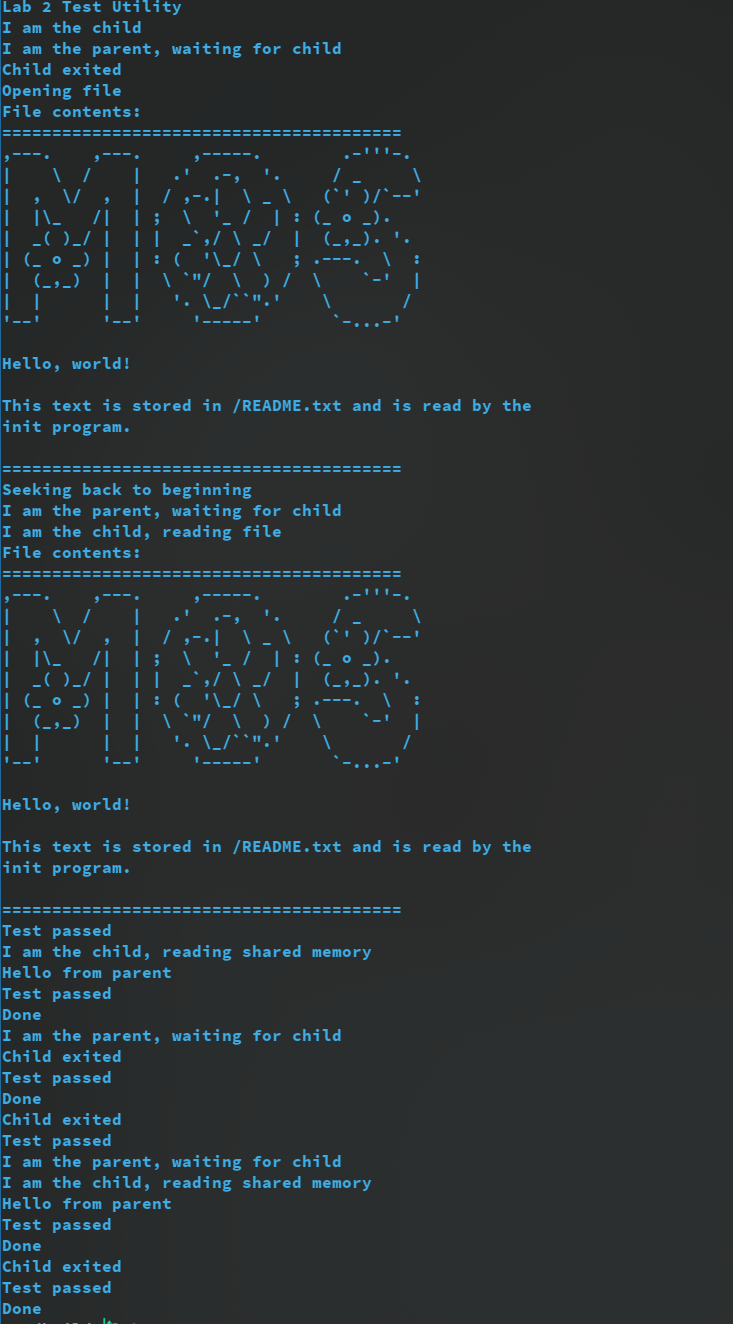
\includegraphics[width=0.8\textwidth]{assets/c2.lab2.png}
    \caption{The output of \texttt{lab2.1}}
    \label{fig:lab2.1-fork}
\end{figure}

If you see a kernel panic saying:

\begin{minted}{text}
    Assertion failed: block.address_space.pgd == process->pagetable.pgd
\end{minted}

Then it means that you have not copied the memory layout correctly.
Pay special attention on the \texttt{vmblock\_t} structure.


\end{document}
